\documentclass[11pt,a4paper]{article}

\usepackage[a4paper,margin=1in]{geometry}
\usepackage[T1]{fontenc}
\usepackage[utf8]{inputenc}
\usepackage{lmodern}
\usepackage{setspace}
\usepackage{parskip}
\usepackage{graphicx}
\usepackage{xcolor}
\usepackage{hyperref}
\usepackage{enumitem}
\usepackage{booktabs}

\hypersetup{
  colorlinks=true,
  linkcolor=black,
  urlcolor=blue,
  citecolor=black,
  pdftitle={CW3 SE Report Group 22}
}

\setstretch{1.08}
\setlist[itemize]{topsep=4pt,itemsep=2pt,leftmargin=1.6em}

\title{\textbf{CW3 SE Report Group 22}}
\author{}
\date{}

\begin{document}

\maketitle
\thispagestyle{empty}

\begin{center}
  Anonymous submission for the SE component of Coursework 3.
\end{center}

\vspace{1em}

\section{Task 1: Design Choices and Implementation Notes}

\subsection{Implemented Use Cases}

This submission implements these use cases:
\begin{itemize}
  \item Log in
  \item Log out
  \item Register entertainment provider
  \item Create event
  \item Search for performances
  \item View performance
  \item Book performance
  \item Edit preferences
  \item Cancel performance
  \item Cancel booking
\end{itemize}

\subsection{System Structure}

The implementation follows the structure suggested by the coursework diagrams. The
\texttt{controller} package contains the use-case logic: \texttt{UserController} handles
authentication, registration, and student preferences; \texttt{EventPerformanceController}
handles event creation, search, viewing, and performance cancellation; and
\texttt{BookingController} handles booking and booking cancellation. The
\texttt{MenuController} provides the top-level text-menu flow and dispatches to the
three main controllers depending on the current user role.

The \texttt{model} package stores the main domain objects, including \texttt{User} and
its subtypes, \texttt{Event}, \texttt{Performance}, \texttt{Booking}, and
\texttt{StudentPreferences}. The \texttt{view} package provides a text-based interface
through the \texttt{View} abstraction and \texttt{TextUserInterface} implementation.
The \texttt{integration} package adapts the provided external verification API to the
names used in the UML. During execution, application data is stored in shared in-memory
collections for users, events, performances, and bookings, which are passed to the
controllers from \texttt{Main}.

\subsection{Alignment with the Provided UML}

The implementation was written to stay close to the supplied UML, but a few points
required small adjustments. First, some APIs shown in the class diagram belong to
four-person-group use cases such as \texttt{reviewPerformance()} and
\texttt{sponsorPerformance()}. Because our group size is three, we kept these methods as
documented placeholders rather than removing them, but left them unimplemented with
explicit comments explaining why.

Second, some data access in the sequence diagrams is more abstract than a concrete Java
implementation. For example, refund processing for \texttt{Cancel performance} is shown
through \texttt{getBookingDetailsForRefund()}, so the controller follows this interface
and parses refund details from the returned value before calling the payment system.
However, local state updates still need direct booking objects afterwards. If we were to
revise the UML, we would clarify which helper methods are intended as public workflow
APIs and which are only abstract descriptions of internal data flow.

\subsection{Key Design Choices}

One important design choice was to keep controller responsibilities narrow and explicit.
Each controller is responsible for a coherent set of use cases, while the model classes
hold the data and small pieces of domain logic such as ticket availability, booking
status, or preference matching. Shared parsing and validation logic was moved into
\texttt{InputParsers} so that the same input rules are reused across multiple use cases.

Another important choice was to maintain shared application collections for events,
performances, bookings, and users. This made it easier to match the use-case flow in
the sequence diagrams and to write system tests that exercise multiple use cases in
sequence. We also separated the text interface behind the \texttt{View} interface so
that real console interaction and scripted system tests could use the same controller
logic.

\subsection{Quality Considerations in the Implementation}

We focused most on reliability and input robustness. User-entered values are validated
close to the point of entry, and several use cases follow the wording of the requirements
by retrying only where the document says they should retry and terminating otherwise.
This reduces the chance of moving the system into invalid states. We also made payment
and refund flows explicit, including the booking states \texttt{ACTIVE},
\texttt{PAYMENTFAILED}, \texttt{CANCELLEDBYSTUDENT}, and
\texttt{CANCELLEDBYPROVIDER}.

We also addressed security in a limited but concrete way by storing user passwords as
salted hashes rather than plain text, including for preregistered users loaded from file.
Finally, maintainability was supported by adding Javadoc, keeping tests aligned with use
cases, and automating formatting, testing, packaging, report generation, and Javadoc
generation through Maven, pre-commit, and GitHub Actions.

\newpage

\section{Task 5: Reflection}

\subsection{Reflection on Teamwork}

\noindent

\textbf{The Experience}
Our team organised the implementation around GitHub pull requests rather than direct commits to the main branch. We created feature branches, opened pull requests for all changes, and used automated checks before review and merge. We also agreed early on the controller and model interfaces so that different use cases could be implemented in parallel with fewer clashes. This gave us a predictable workflow for coding, reviewing, and integrating work.

\textbf{Reflection on Action}
This worked well because it reduced accidental breakage and made each change easy to inspect. The required checks on each pull request forced us to keep the project buildable: Maven tests, Java formatting, and LaTeX report generation all had to succeed before merge. Pre-commit automation also pushed formatting and generated report updates back to the pull-request branch, which reduced manual clean-up. Branch protection, required status checks, linear history, blocked force pushes, and squash-and-merge together kept the repository history much cleaner than in previous coursework. The main disadvantage was speed: even small changes took longer because they had to pass the same workflow, and debugging CI failures occasionally delayed progress.

\textbf{Theory}
We learned that strong repository rules can improve teamwork, not just code quality. A pull-request-first workflow gave us both review discipline and a shared understanding of interfaces and integration points.

\textbf{Preparation}
Next time we would keep the same protected-branch workflow, but add a lightweight board for tracking dependencies between use cases so that blocked work is visible earlier and review can be scheduled more evenly.

\subsection{Reflection on the Quality of the Work and Quality Attributes}

\noindent
\textbf{The Experience}
We think the strongest part of our work was the combination of implementation and testing rather than implementation alone. The main three-person-group use cases were built into a working text-based system, then reinforced with unit tests, use-case-specific system tests, menu-level tests, and longer end-to-end chains. We also spent time aligning the code with the supplied UML and later clarifications instead of treating the diagrams as disposable.

\textbf{Reflection on Action}
The quality attribute we addressed most clearly was reliability. We tried to make invalid states and incorrect user actions visible and recoverable through explicit validation, controlled retry loops, and defensive handling of failure branches such as failed payment or refund flows. This was supported by tests for both normal paths and error paths, for example invalid identifiers, unavailable tickets, cancellation rules, and refund edge cases. We also improved reliability of the development process itself by requiring all checks to pass before merge. A second quality attribute was maintainability: controllers, models, view abstractions, utility parsers, CI packaging, and report tooling were all separated so that responsibilities stayed relatively clear.

\newpage

\textbf{Theory}
We learned that quality came less from any single design decision and more from repeatedly tightening mismatches between code, tests, and documentation.

\textbf{Preparation}
With more time, we would measure coverage formally, expand Javadoc further, and remove or refactor more residual placeholder APIs so the final codebase looked less like an extended coursework skeleton and more like a fully finished system.

\subsection{Reflection on Tools, Agile Approaches and Practices}

\noindent
\textbf{The Experience}
We chose GitHub as the centre of the workflow because it combined version control, pull requests, review, and CI in one place. We used Maven for building, testing, and packaging, pre-commit for formatting hooks, and GitHub Actions for automated checks. We also created a LaTeX build workflow so the report PDF was generated automatically instead of maintained manually.

\textbf{Reflection on Action}
This toolchain matched an agile, incremental style of work. Small branches and pull requests allowed us to build use cases one at a time while keeping the system in a releasable state. Automated formatting reduced style arguments, while required checks made test failures visible immediately. The LaTeX workflow was useful because it turned the report into another reproducible build artifact rather than a separate manual task. The strongest practice here was continuous integration combined with branch protection: no direct commits to the protected branch, required checks before merge, squash merge for tidy history, linear history, and blocked force pushes. The downside was overhead. For coursework-scale changes, setting up and maintaining this pipeline took time, and a few CI issues required debugging infrastructure rather than application logic.

\textbf{Theory}
We learned that these tools were most useful when combined as a system: pre-commit, CI, pull requests, and branch protection each reinforced the others.

\textbf{Preparation}
Next time we would keep the same workflow, but add clearer dashboard-style tracking of open tasks and review ownership so that process information is as visible as build information.

\subsection{Screenshots of Tools and Practices}

The screenshots below show the main tools and practices described in the reflection:
pull-request-based development, automated GitHub Actions checks, and repository rules
that enforced protected-branch collaboration.

\begin{figure}[h]
  \centering
  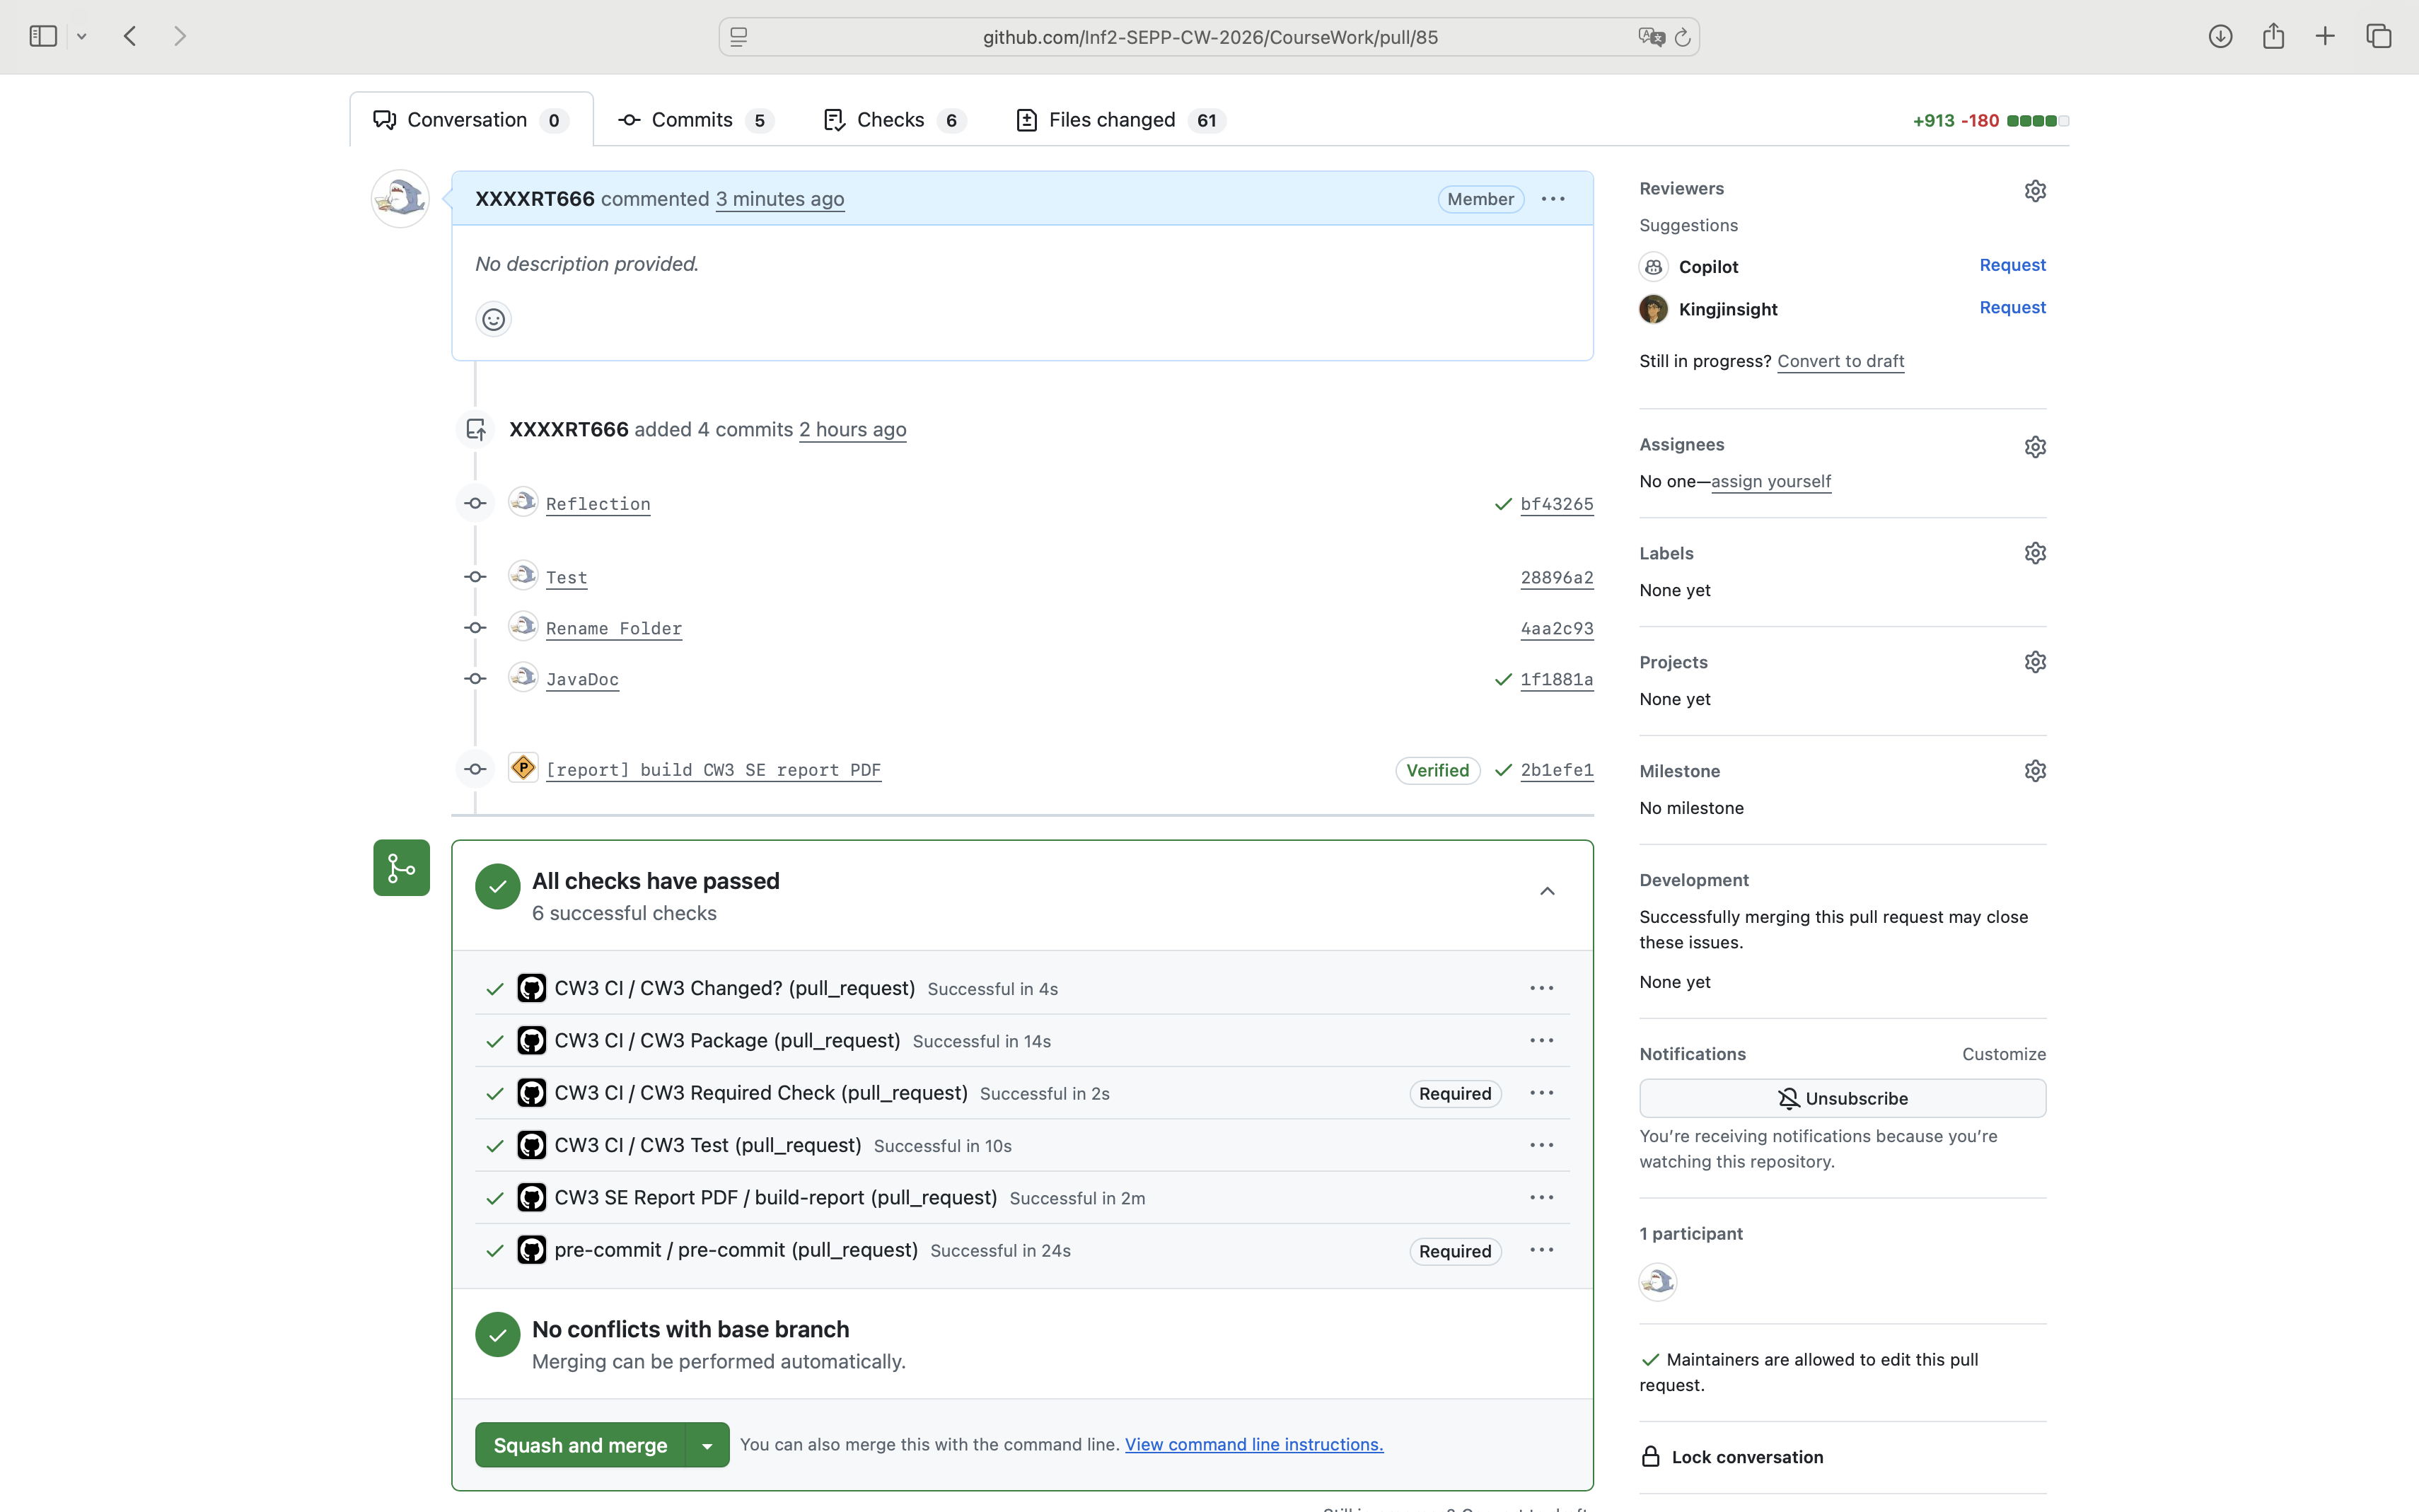
\includegraphics[width=0.92\linewidth]{img3.png}
  \caption{A pull request used for review and integration, showing the required checks and squash-and-merge workflow.}
\end{figure}

\begin{figure}[h]
  \centering
  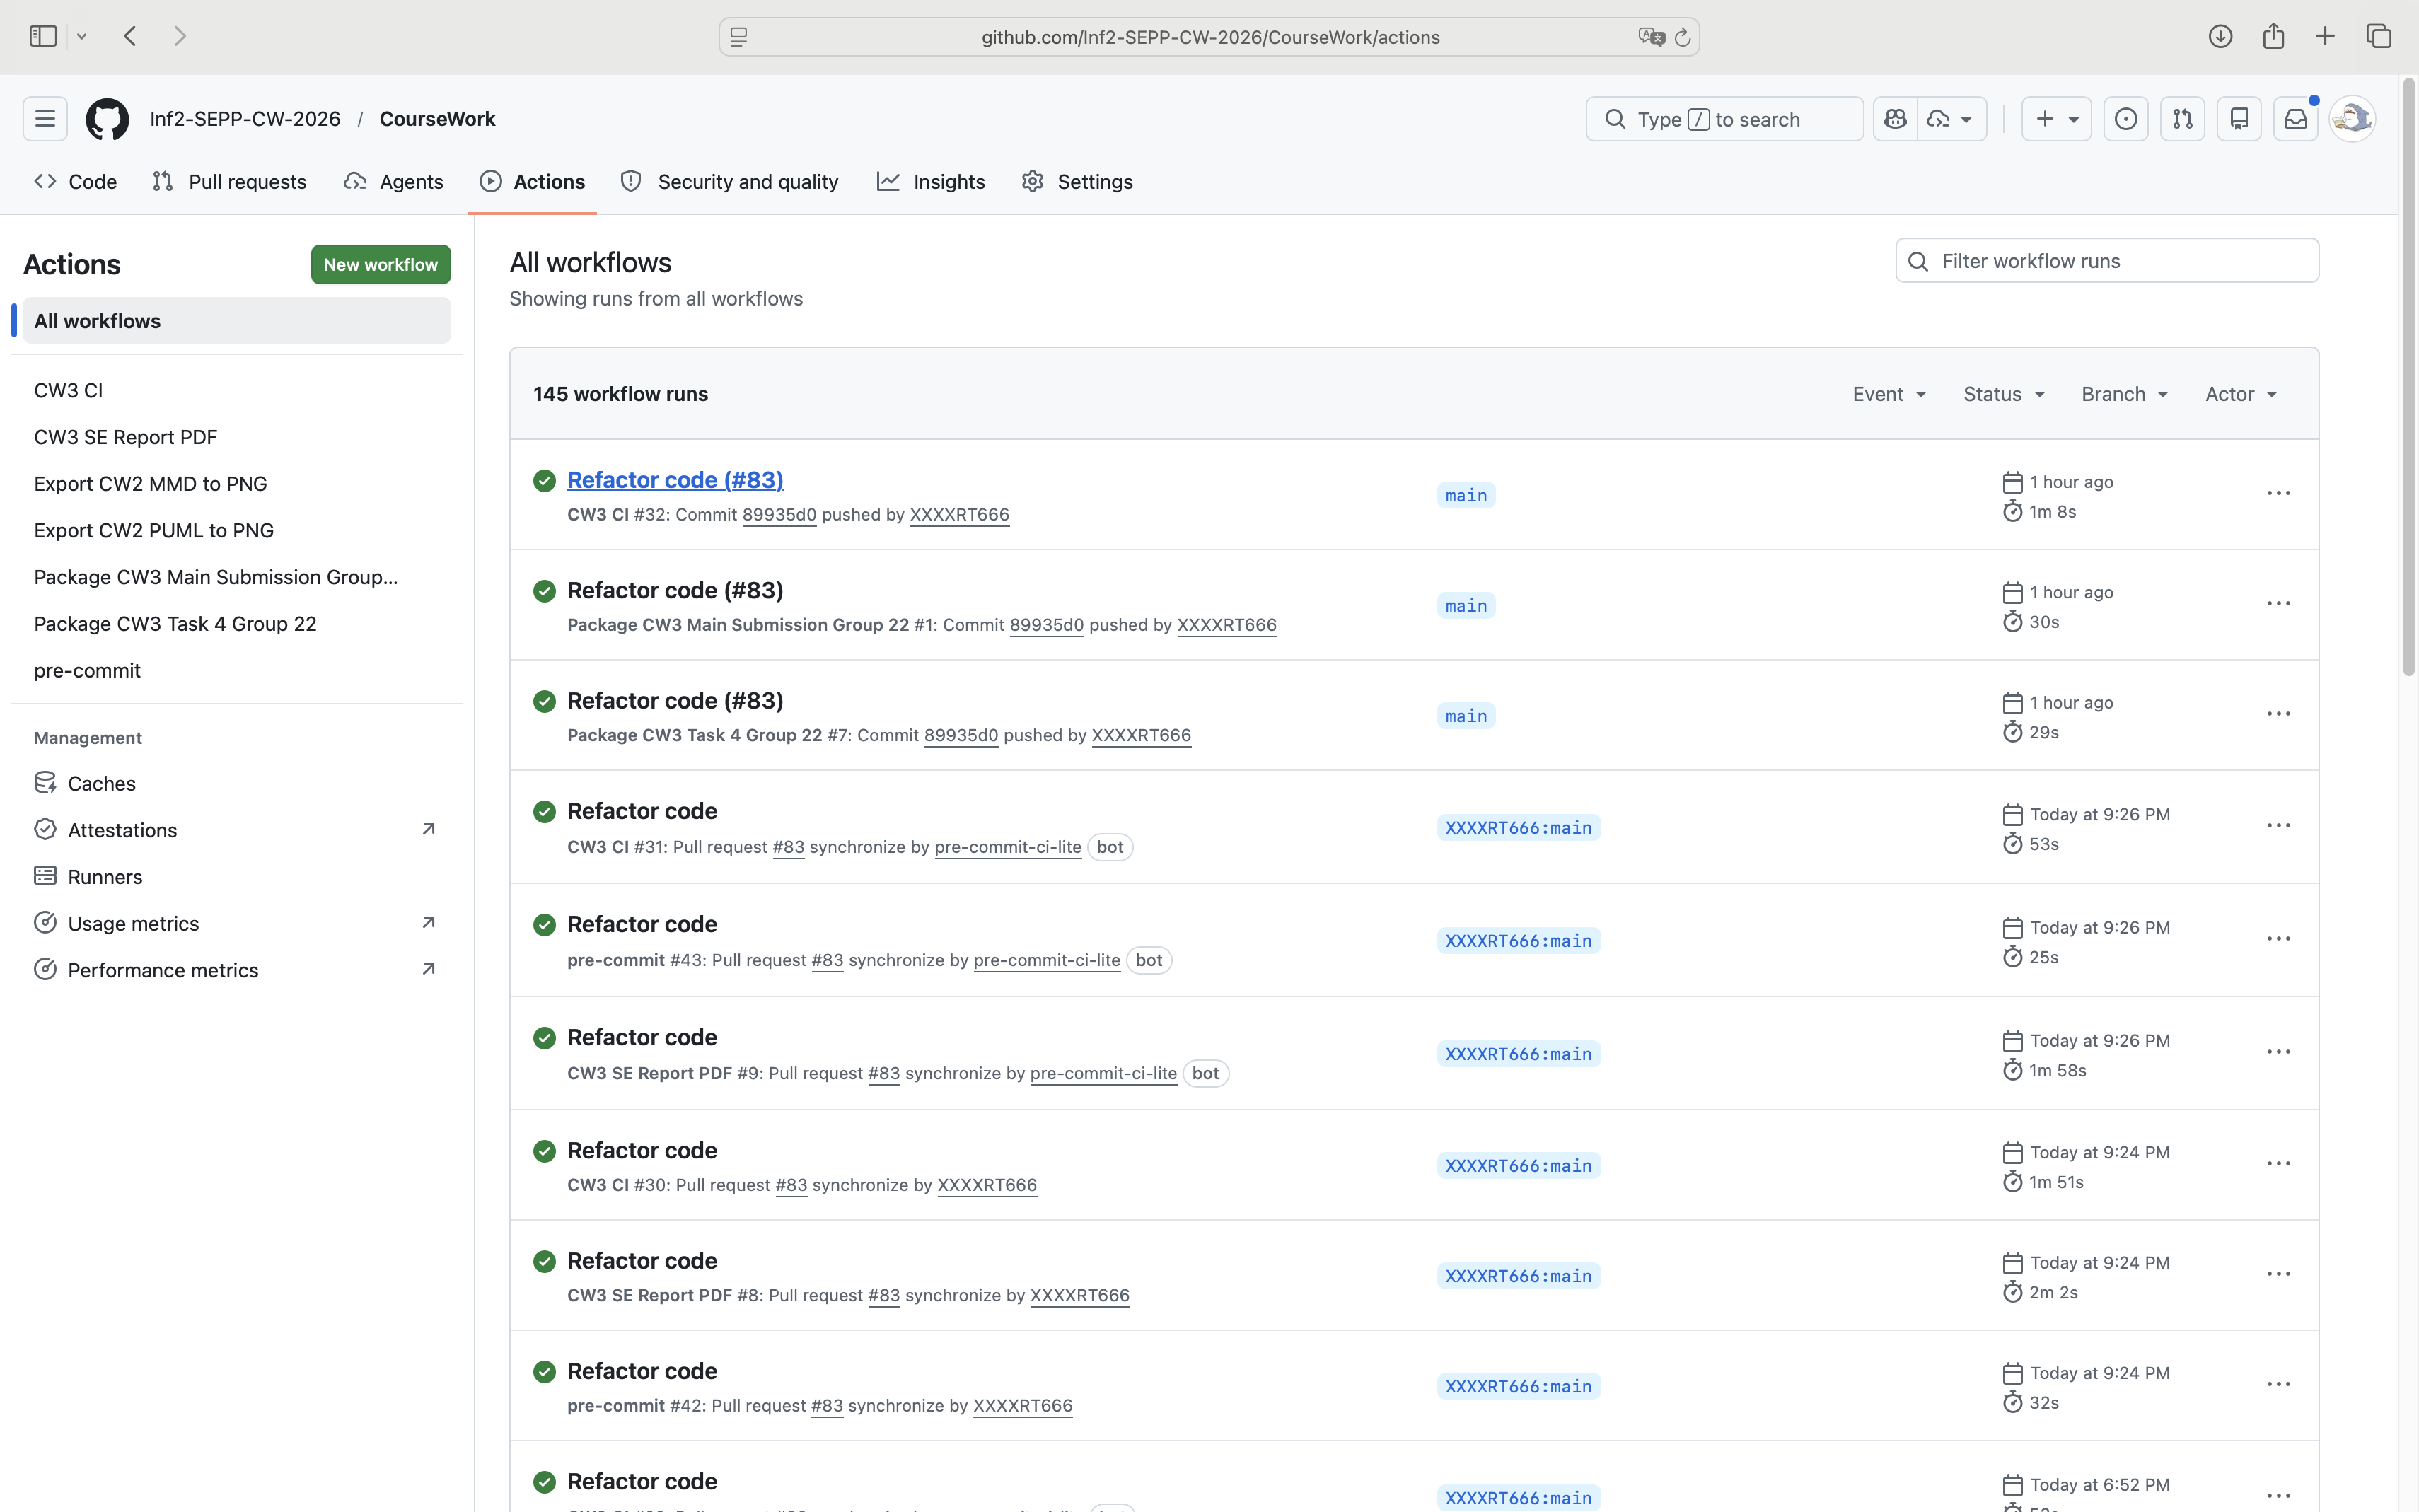
\includegraphics[width=0.92\linewidth]{img1.png}
  \caption{GitHub Actions workflow runs for the repository, including testing, formatting, report generation, and packaging automation.}
\end{figure}

\begin{figure}[h]
  \centering
  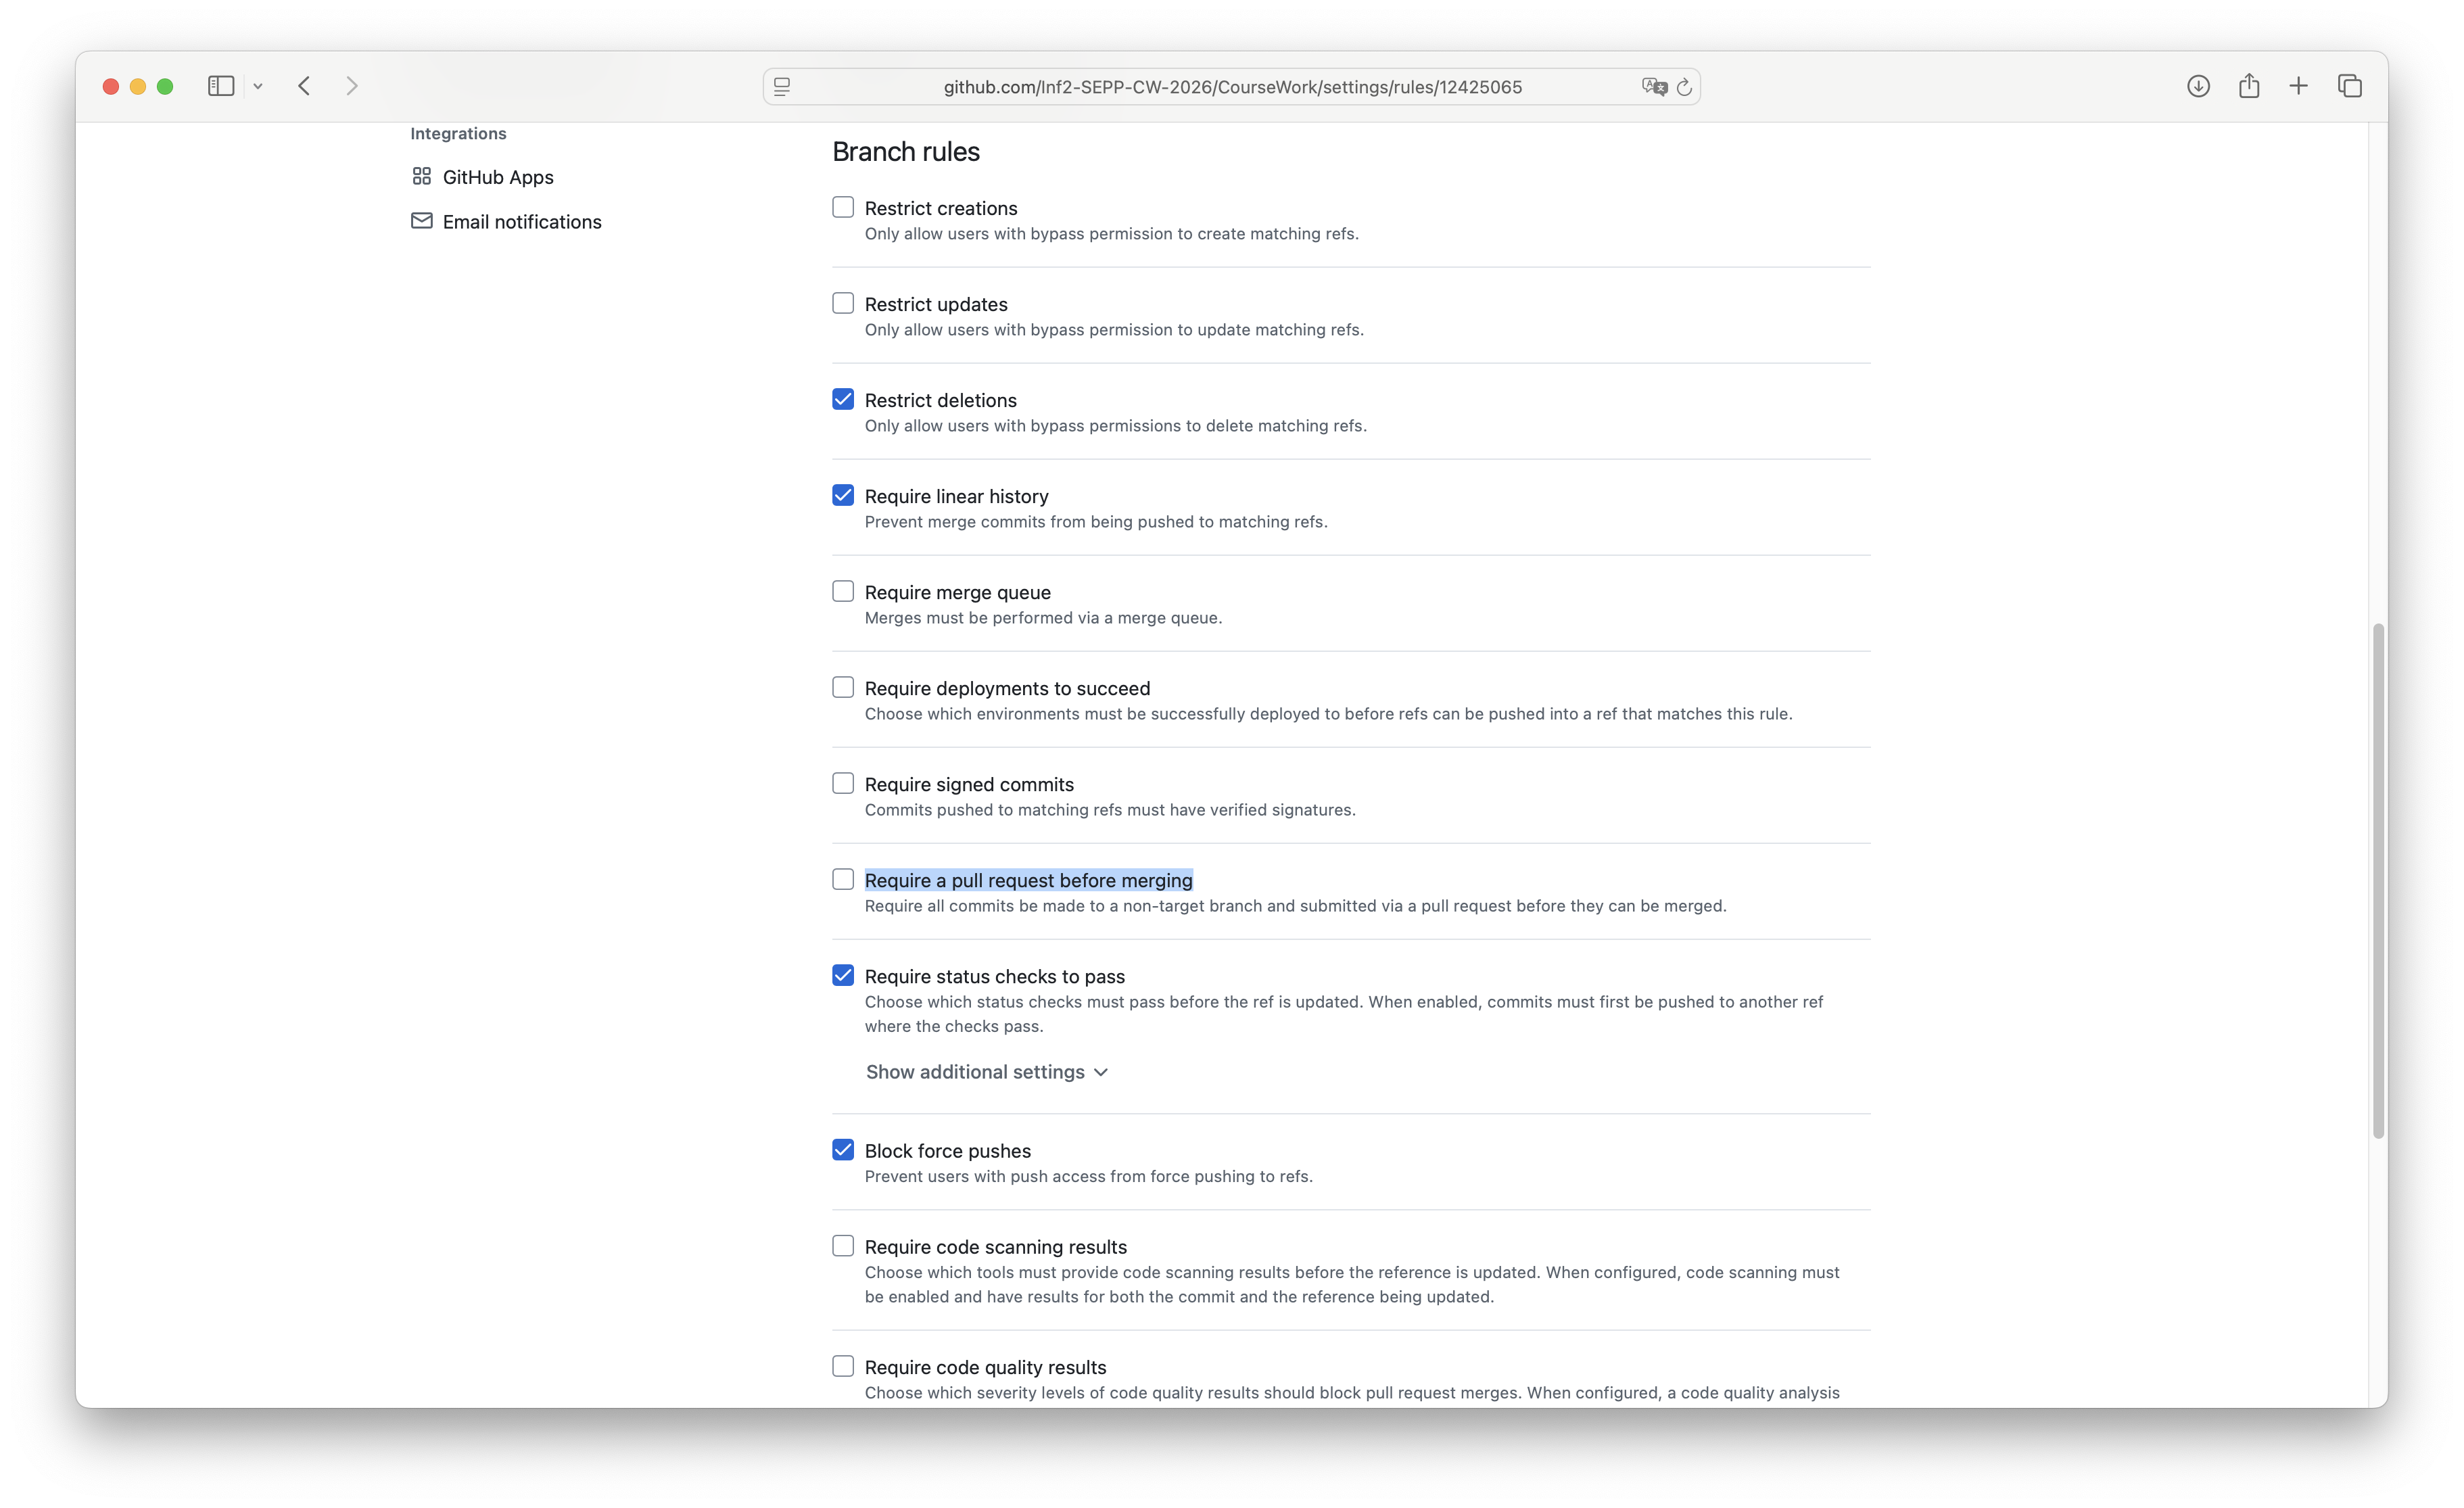
\includegraphics[width=0.92\linewidth]{img5.png}
  \caption{Repository branch protection rules requiring pull requests, passing status checks, linear history, and blocked force pushes.}
\end{figure}

\end{document}
